%%%%%%%%%%%%%%%%%%%%%%%%%%%%%%%%%%%%

\section{モデル選択}

%%%%%%%%%%%%%%%%%%%%%%%%%%%%%%%%%%%%

\subsection{モデル内で有益でない可能性のある変数の識別}

%%%%%%%%%%%%%%%%%%%%%%%%%%%%%%%%%%%

\begin{frame}
\frametitle{教室における美貌}

\begin{itemize}

\item データ：テキサス大学の 463 コースにおける教員の美貌と授業評価の学生評価。

\item 評価は学期末に実施され、美貌の判定はその後、授業に参加しておらず授業評価を知らない 6 人の学生（上位学年の女性 2 人、男性 2 人、下位学年の女性 1 人、男性 1 人）が行った。

\end{itemize}

\ct{Hamermesh \& Parker. (2004)``Beauty in the classroom: instructors? pulchritude and putative pedagogical productivity? Economics Education Review.}

\end{frame}

%%%%%%%%%%%%%%%%%%%%%%%%%%%%%%%%%%%

\begin{frame}
\frametitle{教員評価 vs. 美貌}

教員評価スコア（高いほど良い）vs. 美貌スコア（0 が平均、負が平均以下、正が平均以上）：

\begin{center}
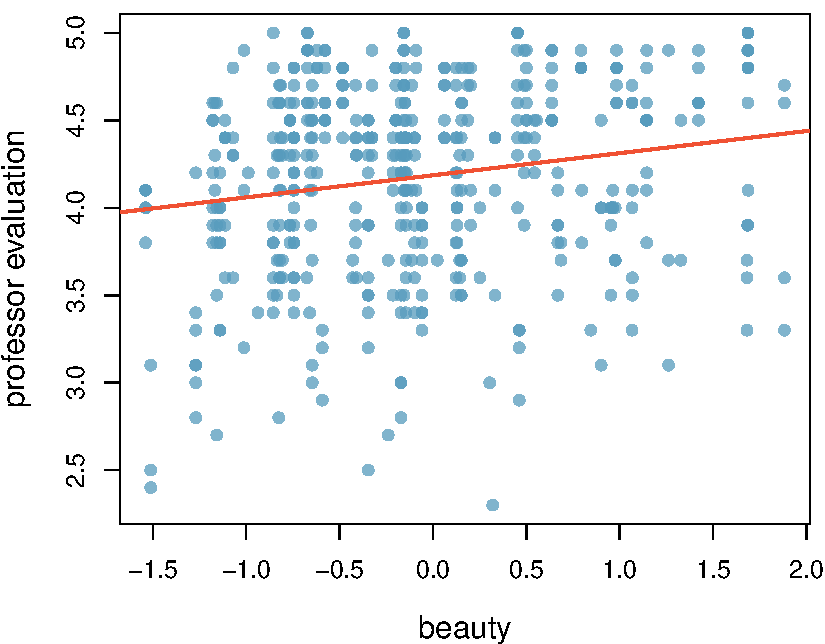
\includegraphics[width=0.65\textwidth]{9-2_model_select/figures/beauty/beauty_profeval}
\end{center}

\end{frame}

%%%%%%%%%%%%%%%%%%%%%%%%%%%%%%%%%%%

\begin{frame}
\frametitle{}

\pq{モデル出力に基づき、以下のうち\underline{正しい}ものはどれか？}

\begin{center}
{\small
\begin{tabular}{rrrrr}
  \hline
 & Estimate & Std. Error & t value & Pr($>$$|$t$|$) \\
  \hline
(Intercept) & 4.19 & 0.03 & 167.24 & 0.00 \\
  beauty & 0.13 & 0.03 & 4.00 & 0.00 \\
   \hline
$R^2$ = 0.0336
\end{tabular}
}
\end{center}

\begin{enumerate}[(a)]
\item このモデルは教員評価の 3.36\% を正確に予測できる。
\item 美貌は教員評価の有意な予測変数ではない。
\solnMult{美貌スコアが平均より 1 点高い教員は、評価も 0.13 点高い傾向がある。}
\item 美貌スコアの変動の 3.36\% は教員評価で説明できる。
\item 相関係数は $\sqrt{0.0336} = 0.18$ または $-0.18$ の可能性があるが、どちらか判別できない。
\end{enumerate}

\end{frame}

%%%%%%%%%%%%%%%%%%%%%%%%%%%%%%%%%%%

\begin{frame}
\frametitle{探索的分析}

\twocol{0.4}{0.6}
{
\dq{興味深い特徴はあるか？}
\soln{美貌スコアが非常に低い女性教員が少ない。}
$\:$ \\
\dq{同じ美貌スコアを持つ場合、男性教員は女性教員より高く評価されるか、低く評価されるか、ほぼ同じか？}
\soln{このプロットだけでは判断が難しい。}
}
{
\begin{center}
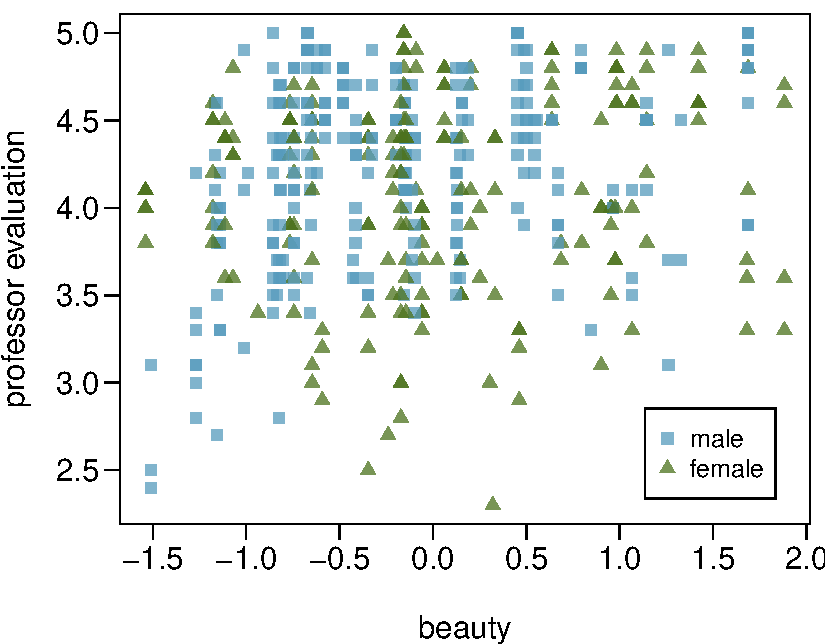
\includegraphics[width=\textwidth]{9-2_model_select/figures/beauty/beauty_profeval_gender}
\end{center}
}

\end{frame}

%%%%%%%%%%%%%%%%%%%%%%%%%%%%%%%%%%

\begin{frame}[fragile]
\frametitle{教員評価 vs. 美貌 + 性別}

\pq{同じ美貌スコアを持つ場合、男性教員は女性教員より高く評価されるか、低く評価されるか、ほぼ同じか？}

{\small
\begin{center}
\begin{tabular}{rrrrr}
  \hline
 & Estimate & Std. Error & t value & Pr($>$$|$t$|$) \\
  \hline
(Intercept) & 4.09 & 0.04 & 107.85 & 0.00 \\
  beauty & 0.14 & 0.03 & 4.44 & 0.00 \\
  gender.male & 0.17 & 0.05 & 3.38 & 0.00 \\
   \hline
$R^2_{adj}$ = 0.057
\end{tabular}
\end{center}
}

\begin{enumerate}[(a)]
\solnMult{高い} \only<2->{\orange{$\rightarrow$ 美貌を一定にすると、男性教員は女性教員より平均 0.17 点高く評価される。}}
\item 低い
\item ほぼ同じ
\end{enumerate}

\end{frame}

%%%%%%%%%%%%%%%%%%%%%%%%%%%%%%%%%%%

\begin{frame}[fragile]
\frametitle{フルモデル}

{\small
\begin{center}
\begin{tabular}{rrrrr}
  \hline
 & Estimate & Std. Error & t value & Pr($>$$|$t$|$) \\
  \hline
(Intercept) & 4.6282 & 0.1720 & 26.90 & 0.00 \\
  beauty & 0.1080 & 0.0329 & 3.28 & 0.00 \\
  gender.male & 0.2040 & 0.0528 & 3.87 & 0.00 \\
  age & -0.0089 & 0.0032 & -2.75 & 0.01 \\
formal.yes \footnote{\texttt{formal}：ネクタイ・ジャケット/ブラウスを着た写真、水準：\texttt{yes}、\texttt{no}} & 0.1511 & 0.0749 & 2.02 & 0.04 \\
  lower.yes \footnote{\texttt{lower}：下位学年のコース、水準：\texttt{yes}、\texttt{no}} & 0.0582 & 0.0553 & 1.05 & 0.29 \\
  native.non english & -0.2158 & 0.1147 & -1.88 & 0.06 \\
  minority.yes & -0.0707 & 0.0763 & -0.93 & 0.35 \\
  students \footnote{\texttt{students}：学生数} & -0.0004 & 0.0004 & -1.03 & 0.30 \\
  tenure.tenure track \footnote{\texttt{tenure}：テニュア状況、水準：\texttt{non-tenure track}、\texttt{tenure track}、\texttt{tenured}} & -0.1933 & 0.0847 & -2.28 & 0.02 \\
  tenure.tenured & -0.1574 & 0.0656 & -2.40 & 0.02 \\
   \hline
\end{tabular}
\end{center}
}

\end{frame}

%%%%%%%%%%%%%%%%%%%%%%%%%%%%%%%%%%%

\begin{frame}
\frametitle{仮説}

傾きパラメータの解釈がモデル内の他の変数を考慮に入れるように、予測変数の有意性をテストするための仮説も他の変数を考慮に入れる。

$\:$ \\

\begin{itemize}
\item[] \mathhl{H_0:} 他の説明変数がモデルに含まれるとき、$B_i = 0$。
\item[] \mathhl{H_A:} 他の説明変数がモデルに含まれるとき、$B_i \ne 0$。
\end{itemize}

\end{frame}

%%%%%%%%%%%%%%%%%%%%%%%%%%%%%%%%%%%

\begin{frame}
\frametitle{有意性の評価：数値変数}

\pq{年齢の p 値が 0.01 である。これは何を意味するか？}

{\scriptsize
\begin{center}
\begin{tabular}{rrrrr}
  \hline
 & Estimate & Std. Error & t value & Pr($>$$|$t$|$) \\
  \hline
...\\
  age & -0.0089 & 0.0032 & -2.75 & 0.01 \\
...\\
   \hline
\end{tabular}
\end{center}
}

\begin{enumerate}[(a)]
\item p 値が正なので、教員の年齢が高いほど評価も高いと予測される。
\solnMult{他の変数をモデルに保ったとき、教員の年齢が評価と関連しているという強い証拠がある。}
\item 年齢の真の傾きパラメータが 0 である確率は 0.01 である。
\item 年齢の真の傾きパラメータが -0.0089 である確率が約 1\% ある。
\end{enumerate}

\end{frame}

%%%%%%%%%%%%%%%%%%%%%%%%%%%%%%%%%%%

\begin{frame}[fragile]
\frametitle{有意性の評価：カテゴリ変数}

\pq{{\small テニュアは 3 水準のカテゴリ変数（non tenure track、tenure track、tenured）である。以下のモデル出力に基づき、\underline{誤り}はどれか？}}

{\footnotesize
\begin{center}
\begin{tabular}{rrrrr}
  \hline
 & Estimate & Std. Error & t value & Pr($>$$|$t$|$) \\
  \hline
... \\
  tenure.tenure track & -0.1933 & 0.0847 & -2.28 & 0.02 \\
  tenure.tenured & -0.1574 & 0.0656 & -2.40 & 0.02 \\
   \hline
\end{tabular}
\end{center}
}

\begin{enumerate}[(a)]
\item 参照水準は non tenure track である。
\item 他の条件が等しい場合、tenure track の教員は non-tenure track の教員より平均 0.19 点低く評価される。
\item 他の条件が等しい場合、tenured の教員は non-tenure track の教員より平均 0.16 点低く評価される。
\solnMult{他の条件が等しい場合、tenure track と tenured の教員の平均評価には有意な差がある。}
\end{enumerate}

\end{frame}

%%%%%%%%%%%%%%%%%%%%%%%%%%%%%%%%%%%

\begin{frame}
\frametitle{有意性の評価}

\dq{教員の評価スコアの有意な予測変数ではない可能性があるなど、モデルへの貢献が少ないと思われる予測変数はどれか？}

{\scriptsize
\begin{center}
\begin{tabular}{rrrrr}
  \hline
 & Estimate & Std. Error & t value & Pr($>$$|$t$|$) \\
  \hline
(Intercept) & 4.6282 & 0.1720 & 26.90 & 0.00 \\
  beauty & 0.1080 & 0.0329 & 3.28 & 0.00 \\
  gender.male & 0.2040 & 0.0528 & 3.87 & 0.00 \\
  age & -0.0089 & 0.0032 & -2.75 & 0.01 \\
  formal.yes & 0.1511 & 0.0749 & 2.02 & 0.04 \\
  \rowcolor{oiB!50}
  lower.yes & 0.0582 & 0.0553 & 1.05 & 0.29 \\
    \rowcolor{oiB!50}
  native.non english & -0.2158 & 0.1147 & -1.88 & 0.06 \\
    \rowcolor{oiB!50}
  minority.yes & -0.0707 & 0.0763 & -0.93 & 0.35 \\
    \rowcolor{oiB!50}
  students & -0.0004 & 0.0004 & -1.03 & 0.30 \\
  tenure.tenure track & -0.1933 & 0.0847 & -2.28 & 0.02 \\
  tenure.tenured & -0.1574 & 0.0656 & -2.40 & 0.02 \\
   \hline
\end{tabular}
\end{center}
}

\end{frame}

%%%%%%%%%%%%%%%%%%%%%%%%%%%%%%%%%%%

\subsection{2つのモデル選択戦略}

%%%%%%%%%%%%%%%%%%%%%%%%%%%%%%%%%%%

\begin{frame}
\frametitle{モデル選択戦略}

\dq{これまでに学んだことを踏まえ、どの変数をモデルに保ち、どれを除くかを決めるために使える方法をいくつか考えてみよ。}

\end{frame}


%%%%%%%%%%%%%%%%%%%%%%%%%%%%%%%%%%%

\begin{frame}
\frametitle{後退消去法}

\begin{enumerate}

\item フルモデルから始める
\item 1つの変数を除いて各小モデルの $R^2_{adj}$ を記録する
\item $R^2_{adj}$ が最も大きく増加したモデルを選ぶ
\item いずれのモデルも $R^2_{adj}$ が増加しなくなるまで繰り返す

\end{enumerate}

\end{frame}

%%%%%%%%%%%%%%%%%%%%%%%%%%%%%%%%%%%

\begin{frame}[shrink]
\frametitle{後退消去法}

\vspace{-0.3cm}

{\tiny
\begin{tabular}{l | l | c}
フル		& beauty + gender + age + formal + lower + native + minority + students + tenure & \orange{0.0839} \\
\hline
ステップ1 	& gender + age + formal + lower + native + minority + students + tenure		& 0.0642 \\
		& beauty + age + formal + lower + native + minority + students + tenure		& 0.0557 \\
		& beauty + gender + formal + lower + native + minority + students + tenure	& 0.0706 \\
		& beauty + gender + age + lower + native + minority + students + tenure		& 0.0777 \\
		& beauty + gender + age + formal + native + minority + students + tenure		& 0.0837 \\
		& beauty + gender + age + formal + lower + minority + students + tenure		& 0.0788 \\
		& beauty + gender + age + formal + lower + native + students + tenure		& \orange{0.0842} \\
		& beauty + gender + age + formal + lower + native + minority + tenure		& 0.0838 \\
		& beauty + gender + age + formal + lower + native + minority + students		& 0.0733 \\
\hline
ステップ2	& gender + age + formal + lower + native + students + tenure 				& 0.0647 \\
		& beauty + age + formal + lower + native + students + tenure 				& 0.0543 \\
		& beauty + gender + formal + lower + native + students + tenure 			& 0.0708 \\
		& beauty + gender + age + lower + native + students + tenure 				&0.0776  \\
		& beauty + gender + age + formal + native + students + tenure 			& \orange{0.0846} \\
		& beauty + gender + age + formal + lower + native + tenure 				& 0.0844 \\
		& beauty + gender + age + formal + lower + native + students 				& 0.0725 \\
\hline
ステップ3	& gender + age + formal + native + students + tenure 					& 0.0653 \\
		& beauty + age + formal + native + students + tenure					& 0.0534 \\
		& beauty + gender + formal + native + students + tenure					& 0.0707 \\
		& beauty + gender + age + native + students + tenure					& 0.0786 \\
		& beauty + gender + age + formal + students + tenure					& 0.0756 \\
		& beauty + gender + age + formal + native + tenure						& \orange{0.0855} \\
		& beauty + gender + age + formal + native + students					& 0.0713 \\
\hline
ステップ4	& gender + age + formal + native + tenure 							& 0.0667 \\
		& beauty + age + formal + native + tenure								& 0.0553 \\
		& beauty + gender + formal + native + tenure							& 0.0723 \\
		& beauty + gender + age + native + tenure							& 0.0806 \\
		& beauty + gender + age + formal + tenure							& 0.0773 \\
		& beauty + gender + age + formal + native							& 0.0713 \\
\end{tabular}
}

\end{frame}

%%%%%%%%%%%%%%%%%%%%%%%%%%%%%%%%%%%

\begin{frame}[fragile]
\frametitle{R の \texttt{step} 関数}

R の \texttt{step} 関数は同様の後退消去プロセスを行うが、
モデル選択に $R^2_{adj}$ の代わりに AIC（赤池情報量基準）という
異なる指標を使用する。

{\tiny
\begin{verbatim}
Call:
lm(formula = profevaluation ~ beauty + gender + age + formal +
    native + tenure, data = d)

Coefficients:
       (Intercept)              beauty          gendermale
          4.628435            0.105546            0.208079
               age           formalyes   nativenon english
         -0.008844            0.132422           -0.243003
tenuretenure track       tenuretenured
         -0.206784           -0.175967
\end{verbatim}
}

最良モデル：beauty + gender + age + formal + native + tenure

\end{frame}

%%%%%%%%%%%%%%%%%%%%%%%%%%%%%%%%%%%

\begin{frame}
\frametitle{前進選択法}

\begin{enumerate}

\item 応答変数 vs. 各説明変数の回帰から始める
\item $R^2_{adj}$ が最も高いモデルを選ぶ
\item 残りの変数を1つずつ既存のモデルに追加し、$R^2_{adj}$ が最も高いモデルを選ぶ
\item 残りの変数を追加しても $R^2_{adj}$ が増加しなくなるまで繰り返す

\end{enumerate}

\end{frame}

%%%%%%%%%%%%%%%%%%%%%%%%%%%%%%%%%%%

\subsection{自由度調整済み $R^2$ の代替としての p 値アプローチ}

%%%%%%%%%%%%%%%%%%%%%%%%%%%%%%%%%%%

\begin{frame}
\subsection{後退消去法と前進選択法}

\begin{itemize}

\item p 値アプローチによる後退消去法：
\begin{enumerate}
\item フルモデルから始める
\item p 値が最も高い変数を除いて小さいモデルを再適合する
\item モデルに残っているすべての変数が有意になるまで繰り返す
\end{enumerate}

\item p 値アプローチによる前進選択法：
\begin{enumerate}
\item 応答変数 vs. 各説明変数の回帰から始める
\item 最も低い有意な p 値を持つ変数を選ぶ
\item 残りの変数を1つずつ既存のモデルに追加し、最も低い有意な p 値を持つ変数を選ぶ
\item 残りの変数が有意な p 値を持たなくなるまで繰り返す
\end{enumerate}

\end{itemize}

\end{frame}

%%%%%%%%%%%%%%%%%%%%%%%%%%%%%%%%%%%

\begin{frame}
\frametitle{後退消去法：p 値アプローチ}

\resizebox{\textwidth}{!}{%
{\tiny
\begin{tabular}{l | rrrrrrrrrr }
\textbf{ステップ}		& \multicolumn{10}{c}{ \textbf{含まれる変数とp値} } \\
\hline
フル		& beauty	& gender		& age	& formal		& lower 	& native	 	& minority		& students	& tenure		& tenure \\
		& 		& male		& 		& yes		& yes	 & nonenglish	& yes		& 			& tenure track	& tenured \\
		&  0.00 	&  0.00 		& 0.01	& 0.04		& 0.29	& 0.06		& \orange{0.35}	& 0.30		& 0.02		& 0.02 \\
\hline
ステップ1	& beauty	& gender		& age	& formal		& lower 		& native	 	& 			& students	& tenure		& tenure \\
		& 		& male		& 		& yes		& yes		& nonenglish	& 			& 			& tenure track	& tenured \\
		&  0.00 	&  0.00 		& 0.01	& 0.04		& \orange{0.38}	& 0.03		&			& 0.34		& 0.02		& 0.01 \\
\hline
ステップ2	& beauty	& gender		& age	& formal		& 	 		& native	 	& 			& students	& tenure		& tenure \\
		& 		& male		& 		& yes		& 			& nonenglish	& 			& 			& tenure track	& tenured \\
		&  0.00 	&  0.00 		& 0.01	& 0.05		& 			& 0.02		&			& \orange{0.44}	& 0.01		& 0.01 \\
\hline
ステップ3 	& beauty	& gender		& age	& formal		& 	 		& native	 	& 			& 			& tenure		& tenure \\
		& 		& male		& 		& yes		& 			& nonenglish	& 			& 			& tenure track	& tenured \\
		&  0.00 	&  0.00 		& 0.01	& \orange{0.06}	& 			& 0.02		&			& 			& 0.01		& 0.01 \\
\hline
ステップ4	& beauty	& gender		& age	& 			& 	 		& native	 	& 			& 			& tenure		& tenure \\
		& 		& male		& 		& 			& 			& nonenglish	& 			& 			& tenure track	& tenured \\
		&  0.00 	&  0.00 		& 0.01	&			& 			& \orange{0.06}	&			& 			& 0.01		& 0.01 \\
\hline
ステップ5 	& beauty	& gender		& age	& 			& 	 		& 		 	& 			& 			& tenure		& tenure \\
		& 		& male		& 		& 			& 			&			& 			& 			& tenure track	& tenured \\
		&  0.00 	&  0.00 		& 0.01	&			& 			& 			&			& 			& 0.01		& 0.01 \\
\end{tabular}
}}

$\:$ \\

最良モデル：beauty + gender + age + tenure

\end{frame}

%%%%%%%%%%%%%%%%%%%%%%%%%%%%%%%%%%%

\begin{frame}
\frametitle{自由度調整済み $R^2$ vs. p 値アプローチ}

\begin{itemize}

\item 2つのアプローチは似ているが、異なるモデルになることがあり、自由度調整済み $R^2$ アプローチの方が最終モデルに含める予測変数が多くなる傾向がある。

\item 予測精度の向上のみが目標であれば $R^2$ を使う。機械学習の応用でよく見られる。

\item 応答変数の統計的に有意な予測変数がどれかを理解することに関心がある場合、または予測精度をわずかに犠牲にしても単純なモデルを作りたい場合は p 値アプローチが好まれる。

\item どのアプローチを使っても、変数選択後の作業はまだ終わっていない --- モデルの条件（仮定）が妥当かどうかを確認する必要がある。

\end{itemize}

\end{frame}

%%%%%%%%%%%%%%%%%%%%%%%%%%%%%%%%%%%
